%%% use twocolumn and 10pt options with the asme2e format
\documentclass[twocolumn,10pt]{asme2e}
\special{papersize=8.5in,11in}
\usepackage{graphicx}
\usepackage{caption}
\usepackage{subcaption}
\usepackage{lipsum}
\usepackage{multicol}

\confshortname{FEDSM 2020}
\conffullname{the ASME 2020 Fluids Engineering Division Summer Meeting}

\confdate{July 12-16}
\confyear{2020}
\confcity{Orlando, Florida}
\confcountry{USA}

\papernum{FEDSM2020-12388}

%%% You need to remove 'DRAFT: ' in the title for the final submitted version.
\title{DRAFT: The Effect of Variying Viscosity in Turbulent Channel Flow}


%%% first author
\author{Victor Coppo Leite
    \affiliation{
	Ken and Mary Alice Lindquist\\Department of Nuclear Engineering\\
	Pennsylvania State University\\
	State College, PA 16801\\
    Email: vbc5085@psu.edu
    }	
}

%%% second author
%%% remove the following entry for single author papers
\author{Elia Merzari
    \affiliation{
	Ken and Mary Alice Lindquist\\Department of Nuclear Engineering\\
	Pennsylvania State University\\
	State College, PA 16801\\
    Email: ebm5153@psu.edu
    }	
}

\begin{document}

\maketitle    

%%%%%%%%%%%%%%%%%%%%%%%%%%%%%%%%%%%%%%%%%%%%%%%%%%%%%%%%%%%%%%%%%%%%%%
\begin{abstract}
{\it In various applications in nuclear engineering and in particular in test reactors, heat removal is carried by single-phase axial flow. In these applications, we observe sharp changes in molecular viscosity while the density presents very limited changes. As a consequence, the Reynolds number increases often by 2-3 folds across the channel, with an inlet value often transitional.  In these conditions, turbulence changes significantly across the length of the channel with redistribution and thinning of the boundary layers. This is different from acceleration as the effect of changes in density is negligible. We aim to characterize in detail this phenomenon. 

In particular Nek5000, a spectral-element computational fluid dynamics (CFD) code, will be used to perform DNS of fluid flow in the transition regime for channel flow with varying viscosity.  We set up a novel benchmark case: the channel is extended in the stream-wise direction up to 20pi. The viscosity is kept constant in the first 4pi region. This inlet region is used as a cyclic region to obtain a fully developed flow profile at the beginning of the ramping region. The ramping region (4pi -20pi) is defined as a transition region where the viscosity is linearly decreased along the channel. The flow is homogenous in the span-wise direction due to the periodic boundary conditions. Due to the cyclic and wall boundary conditions, the flow is non-homogenous in the stream-wise and wall-normal direction respectively.

In this study, specific focus is given to the investigation of turbulence properties and structures in the near-wall region along the flow direction. Detailed turbulence budgets are collected and investigated. As expected, the results show that variation in the Reynolds across a channel does not cause an immediate change in the size of turbulent structures in the ramp region and a delay is in fact observed. Moreover, the results from the present study are compared with a correlation available in the literature for the friction velocity and as a function of the Reynolds-number.}
\end{abstract}

%%%%%%%%%%%%%%%%%%%%%%%%%%%%%%%%%%%%%%%%%%%%%%%%%%%%%%%%%%%%%%%%%%%%%%
\begin{nomenclature}
\entry{A}{You may include nomenclature here.}
\entry{$\nu$}{Viscosity.}
\entry{$x$}{Streamwise direction.}
\entry{$y$}{Vertical direction.}
\entry{$z$}{Spanwise direction.}
\entry{$Re$}{Reynolds number.}
\entry{$Re_{\tau}$}{Friction Reynolds number.}
\entry{$DNS$}{Direct Numerical Simulation.}
\entry{$ANL$}{Argonne National Laboratory.}
\entry{${\tau}_w$}{Shear stress at the wall.}
\entry{$u_{\tau}$}{Friction velocity.}
\entry{$Re_{\tau}$}{Friction Reynolds number.}
\entry{$\delta$}{Height of the turbulence channel.}
\entry{${F_{Ci}}$}{Delayed function of Cases ${i}$=I,II and III.}
\entry{$a$}{Viscosity linear coefficient.}
\entry{$R$}{Relaxing parameter.}
\entry{$C$}{Contractioning parameter.}
\entry{${\delta}_{i}$}{Streamwise position where Region $i$ starts, ${i}$=I,II and III.}
\entry{${\Lambda}$}{Signal contribution in the delayed function.}
\entry{$BLABLABLA$}{Bullshit.}

\entry{$\alpha$}{There are two arguments for each entry of the nomemclature environment, the symbol and the definition.}
\end{nomenclature}

The spacing between abstract and the text heading is two line spaces.  The primary text heading is  boldface in all capitals, flushed left with the left margin.  The spacing between the  text and the heading is also two line spaces.

%%%%%%%%%%%%%%%%%%%%%%%%%%%%%%%%%%%%%%%%%%%%%%%%%%%%%%%%%%%%%%%%%%%%%%
\section*{INTRODUCTION}

A schematic of the turbulence channels simulated are shown in Fig.~\ref{fig:geometry_turbchannel}. In this figure, Regions I, II and III are defined by two planes crossing the channel. A cycling region is implemented within Region I, Fig.~\ref{fig:cycling_region}.
In this problem, the viscosity \(\nu\) is a function of \(x\), i.e., the streamwise distance. This parameter has constants values of \(1E-4\) Pa.s and \(5E-5\) Pa.s along Regions I and III respectively, while in region II it decreases with respect to the inverse of \(x\).

In the present work, three cases varying the length of Region II are studied. Cases I, II and III have their Region II length of respectively \(16\pi\), \(8\pi\) and \(4\pi\). Fig.~\ref{fig:viscosity} shows the plot of the viscosity as a function of \(x\) for each one of these cases and Fig.~\ref{fig:reynolds} shows the plot of the Reynolds number for them.

For all three Cases the inleat flow in Region I is considered to be fully developed with \(Re_{\tau}=550\), i.e., the same conditions as in \cite{hoyas2008}. Periodic condition is considered for the boundaries of the spamwise direction, i.e., \(z\) axis, and finally wall conditions are considered for the boudaries of the vertical direction, i.e., \(y\) axis.

\begin{figure}[!htbp]
	\centering
	\scalebox{0.5}
	{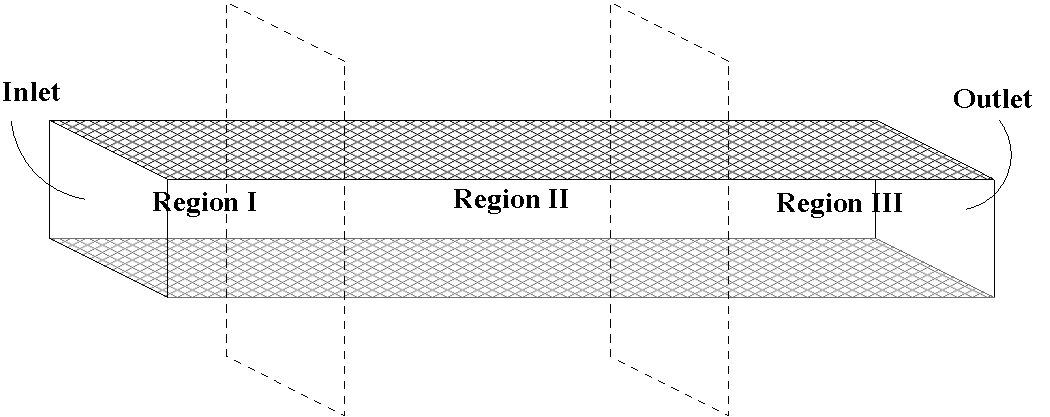
\includegraphics{geometry_turbchannel.pdf}}
	\scalebox{0.4}
	{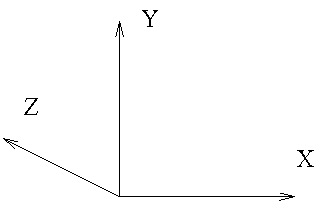
\includegraphics{axis.pdf}}
	\caption{Geometry of the turbulence channel, the channel is divided into three different Regions.}
	\label{fig:geometry_turbchannel}
	\end{figure}

\begin{figure}[!htbp]
	\centering
	\scalebox{0.5}
	{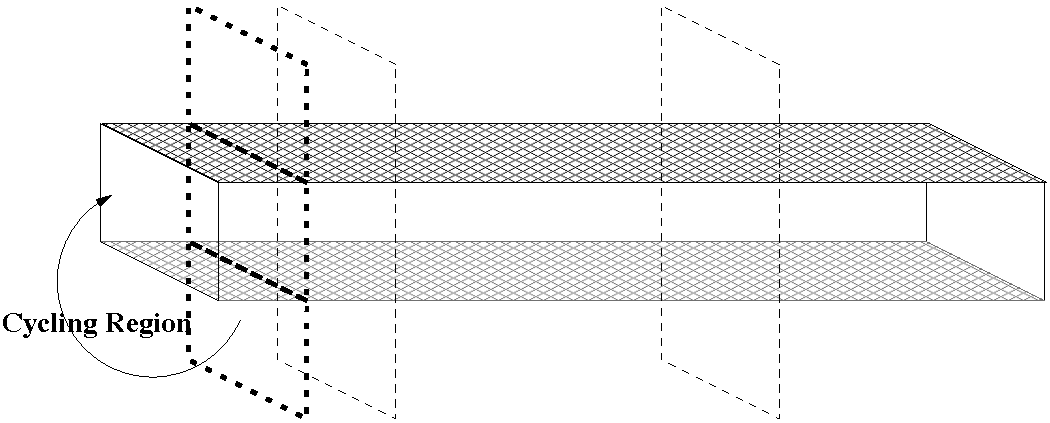
\includegraphics{cycling_region.pdf}}
	\caption{Cyclic region in the inlet.}
	\label{fig:cycling_region}
\end{figure}

\begin{figure}[!htbp]
	\centering
	\scalebox{0.5}
	{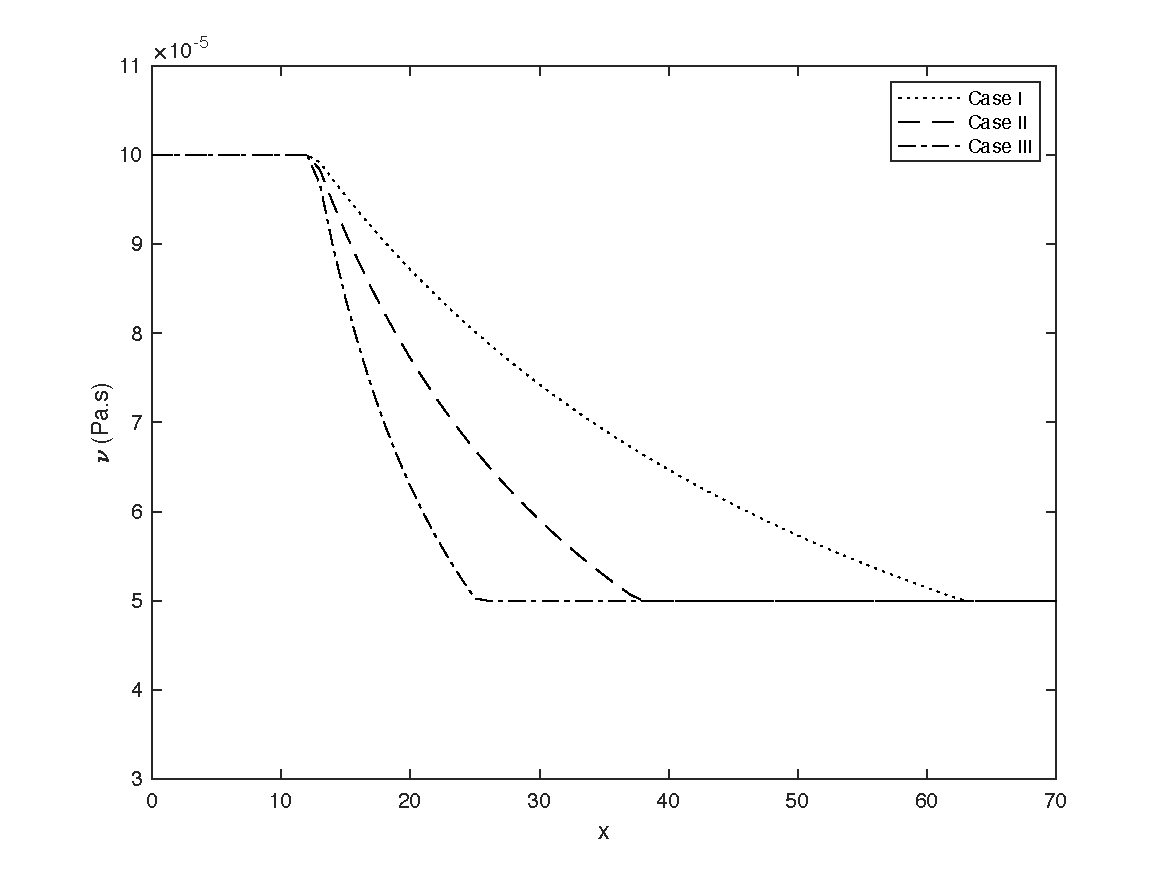
\includegraphics{viscosity.pdf}}
	\caption{The viscosity of the considered Cases as a function of \(x\).}
	\label{fig:viscosity}
	\end{figure}

\begin{figure}[!htbp]
	\centering
	\scalebox{0.5}
	{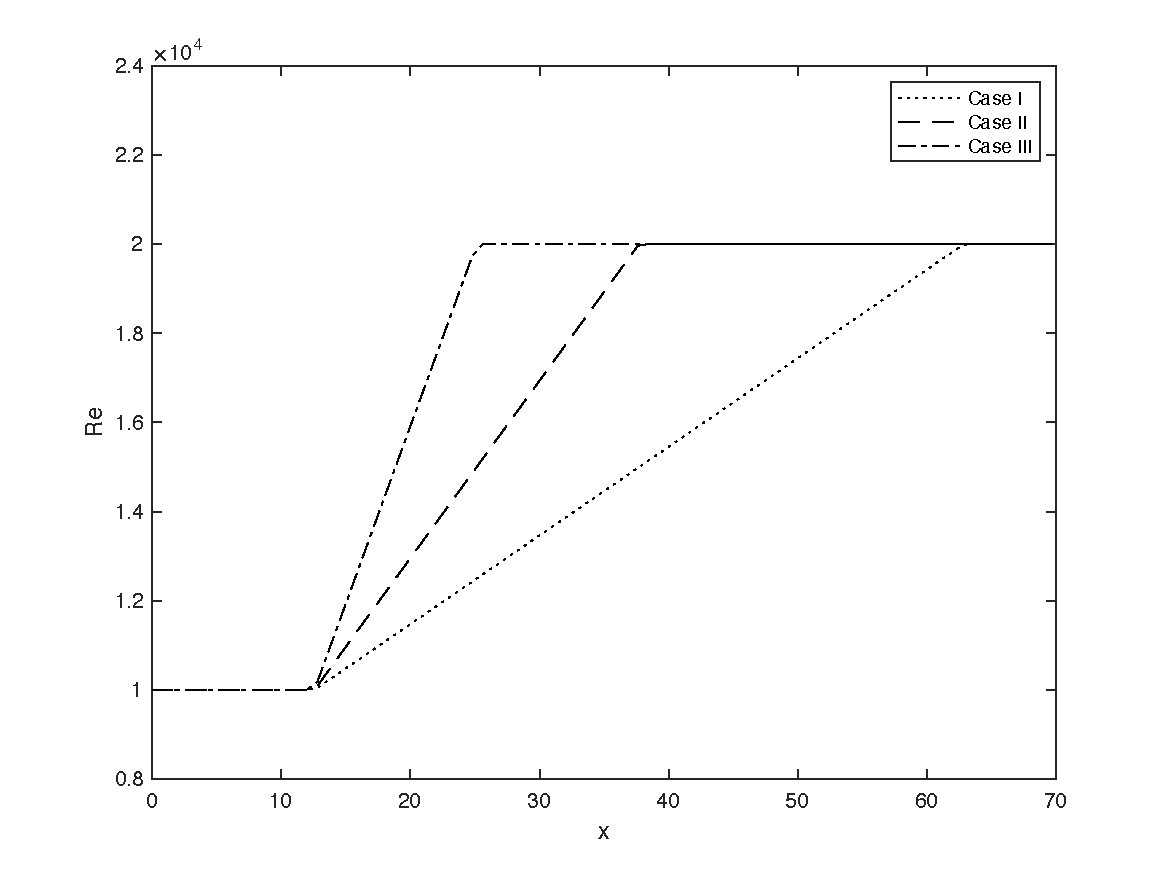
\includegraphics{reynolds.pdf}}
	\caption{The Reynolds number as a function of the \(x\) for the considered Cases.}
	\label{fig:reynolds}
\end{figure}

%%%%%%%%%%%%%%%%%%%%%%%%%%%%%%%%%%%%%%%%%%%%%%%%%%%%%%%%%%%%%%%%%%%%%%
\section*{METHODS - DIRECT NUMERICAL SIMULATION}

In order to resolve the finest turbulent scales, the calculations of this work has been developed through Direct Numerical Simulation (DNS). To do so Nek5000 was employed, a spectral element code developed in Argonne National Laboratory (ANL). Nek5000 has been validated in references \cite{merzari2013} and \cite{Obabko2011}.

The solution of this method is given by trigonometric series, in each element a polynomial functions of up to the twelveth degree have been employed to discretize the velocity field. Fig.~\ref{fig:mesh} shows an example of the grid from half of the channel's cross section. One should notice that the discretization presented by this particular area is identical through all model's domain and it is only presented half of the cross-section for better visualization of the frame.

\begin{figure}[!htbp]
	\centering
	\scalebox{0.16}
	{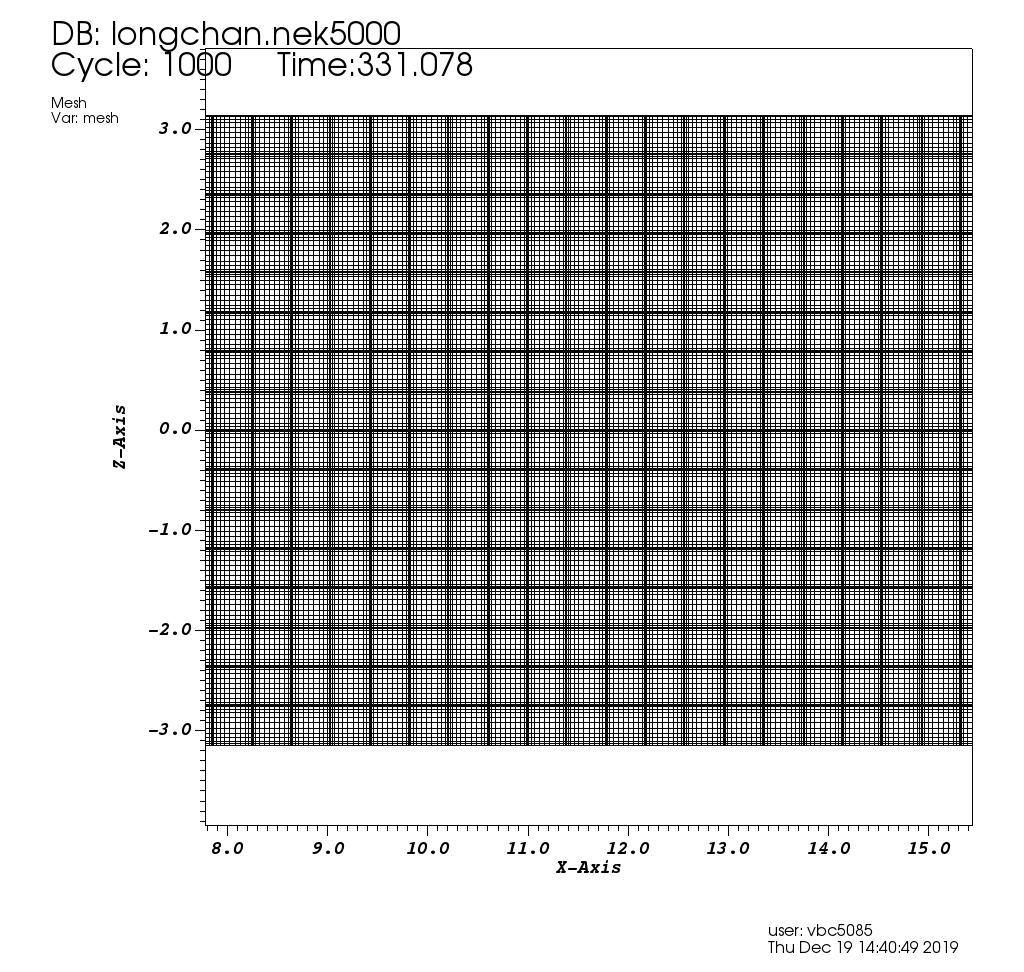
\includegraphics{mesh.png}}
	\caption{The grid employed in the simulation from half of the channel's cross section.}
	\label{fig:mesh}
\end{figure}

DNS simulations are able to simulate the finest turbulent length scales without using any turbulent model. Since the present work is focused on studying the contribution of the smaller scales to the energy cascade, it is required to use DNS rather than Reynolds Average Navier-Stokes (RANS) or Large Eddy Simulations (LES), although there is a substantial growth of the computational cost.

%%%%%%%%%%%%%%%%%%%%%%%%%%%%%%%%%%%%%%%%%%%%%%%%%%%%%%%%%%%%%%%%%%%%%%
\section*{METHODS - CONVOLUTION ANALYSIS OF THE FRICTION REYNOLDS NUMBER}


The friction Reynolds number has been calculated via numerical simulations for Cases I, II and III and this result was compared to the values obtained using an existed expression from Ref.~\cite{pope} valid for fully developed turbulent flows. A delay in space can be seen between \(Re_{\tau}\) when comparing the simulations' results with the values yielded from the mentioned expression. This way, these results are treated as signals in the space and a convolution operation is performed over the analytical expression for fully developed turbulent flows in order to built a function that matches with the obtained values from the simulations.

To calculate the friction Reynolds number from the simulations several velocities profiles along \(x\) were obtained from the results and the viscous stress \(\frac{d<U>}{dy}\) for these locations are calculated. Such values can then be applied in the set of definitions given from Eqn.~\ref{shear_wall} to Eqn.~\ref{friction_reynolds} following presented in order to calculate \(Re_{\tau}\).

\begin{equation}
{\tau}_w = \rho\nu\left(\frac{d<U>}{dy}\right)_{y=0}
\label{shear_wall}
\end{equation}

Where \(\rho\) is the density and \({\tau}_w\)  is the shear stress at the wall.

\begin{equation}
u_{\tau} = \sqrt{\frac{{\tau}_w}{\rho}}
\label{u_t}
\end{equation}

Where \(u_{\tau}\) is the friction velocity. And finally,

\begin{equation}
Re_{\tau} = \frac{u_{\tau}\delta}{\nu}
\label{friction_reynolds}
\end{equation}

Where \(\delta\) is the height of the simulated channels. For all Cases studied here this is a constant parameter \(\delta=2\).

The friction Reynolds number calculated using Eqn.~\ref{friction_reynolds} with the numeric simulations' results is then compared with Eqn.~\ref{reynolds_approximation} from Ref.~\cite{pope}, which is valid for fully developed turbulent flows.

\begin{equation}
Re_{\tau} = 0.09Re^{0.88}
\label{reynolds_approximation}
\end{equation}

The Reynolds numbers used to supply Eqn.~\ref{reynolds_approximation} are those varying through \(x\) from Cases I, II and III, as presented in Fig.~\ref{fig:reynolds}. The convolution to be performed over Eqn.~\ref{reynolds_approximation} is given by Eqn.~\ref{convolution}. In this equation \(Re(\chi)\) stands for the analytical approximation given by Eqn.~\ref{reynolds_approximation}, \(g(x-\chi)\)  is a shifting function and \(\chi\) is simply a dummy variable for the streamwise distance.

\begin{equation}
F(x) =  \int_{-\infty}^{+\infty} Re_{\tau}(\chi)g(x-\chi)d\chi
\label{convolution}
\end{equation}

As mentioned earlier, the simulated channels in the present study are divided in three Regions, as shown in Fig.~\ref{fig:geometries} and a delayed function is built for each one of those. Since there is no delay in Region I, no special treatment is required for it, thus \(F(x)=Re_{\tau}(x)=550\). Differently, in Region II and III the results from the numerical experiments are delayed when compared to those from Eqn.~\ref{reynolds_approximation} and because of that a convolution operator takes place. Since we are dealing with a delayed signal in both Regions, a decaying exponential has been used as a shifting function, as proposed in Ref.~\cite{signals}.

In Region II, the friction Reynolds number is a linear function given by Eqn.~\ref{region2_reynolds}.

\begin{equation}
Re_{\tau}(x)=ax+550
\label{region2_reynolds}
\end{equation}

Where \(a\) is the linear coefficient of the increasing viscosity for each one of the three cases in Region II. Using Eqn.~\ref{region2_reynolds} in conjunction to the definition from Eqn.~\ref{convolution}, one may derive Eqn.~\ref{region2_delayed}, which is the delayed function valid for Region II of the considered Cases.

\begin{equation}
F(x)= \frac{a}{R^2}(e^{-R(x-{\delta}_{II})}-1)+\frac{a}{R}(x-{\delta}_{II})+550
\label{region2_delayed}
\end{equation}

Where \({\delta}_{II}\) is the streamwise position that Region II starts and \(R\) is named relaxing parameter and it stands for the exponential decaying constant to be used in the shifting function \(g(x-\chi)\) when dealing with Region II.

Eqn.~\ref{region3_delayed} is the delayed function yielded applying Eqn.~\ref{convolution} over Region III, where a constant friction Reynolds number \(Re_{\tau}\) predicted by Eqn.~\ref{reynolds_approximation} takes place.

\begin{equation}
F(x)= (20000-{\Lambda})(1-e^{-C(x-{\delta}_{III})})+{\Lambda}
\label{region3_delayed}
\end{equation}

In this equation \({\delta}_{III}\) is the streamwise position that Region III starts, \(C\) is named contractioning parameter and it stands for the exponential decaying constant to be used in the shifting function \(g(x-\chi)\) when dealing with Region III and finally
 \({\Lambda}=\frac{a}{R^2}(e^{-R({\delta}_{III}-{\delta}_{II})}-1)+\frac{a}{R}({\delta}_{III}-{\delta}_{II})+550\), represents the contribution from Regions II to the delayed signal in Region III.

%%%%%%%%%%%%%%%%%%%%%%%%%%%%%%%%%%%%%%%%%%%%%%%%%%%%%%%%%%%%%%%%%%%%%%

\section*{RESULTS}

The results from the three cases considered in this work are presented in this section. First, the friction Reynolds number variation along the streamwise direction \(x\) of the channels are computed and compared with an expression for \(Re_{\tau}\) as a function of the Reynolds number existed in Ref.~\cite{pope}. This analysis shows the fact that the friction Reynolds number due to a viscosity change imposed through region II is not immediate. Thereon, Reynolds stresses are collected and turbulent structures are investigated along the simulated channels.

Fig.~\ref{fig:re_t_x} shows the plot of the friction Reynolds number thourgh \(x\) calculated via CFD analisys and by the analytical Eqn.~\ref{anl_ret} for Case I. In this figure, \(Re_{\tau}\) calculated via DNS is delayed in space when compared to the value obtained using the analytical solution provided by Eqn.~\ref{anl_ret}. This fact shows that the effect of the change in the viscosity doesn't cause an immediate effect on the turbulence of the flow. In this sense, the friction Reynolds number calculated through Eqn.~\ref{anl_ret} can be treated as signal over the space \(x\), and a convolution operation can be performed yielding a delayed signal that can be adjusted so it matches to the simulated results. Furthermore, the function \(F_{CI}(x)\) plotted in graph from Fig.~\ref{fig:re_t_x} is the result of this approach, a detailed description about the steps to derive the convolution functions for this study are provided in the following subsection.

\begin{figure}[!htbp]
\begin{center}
\setlength{\unitlength}{0.012500in}%
  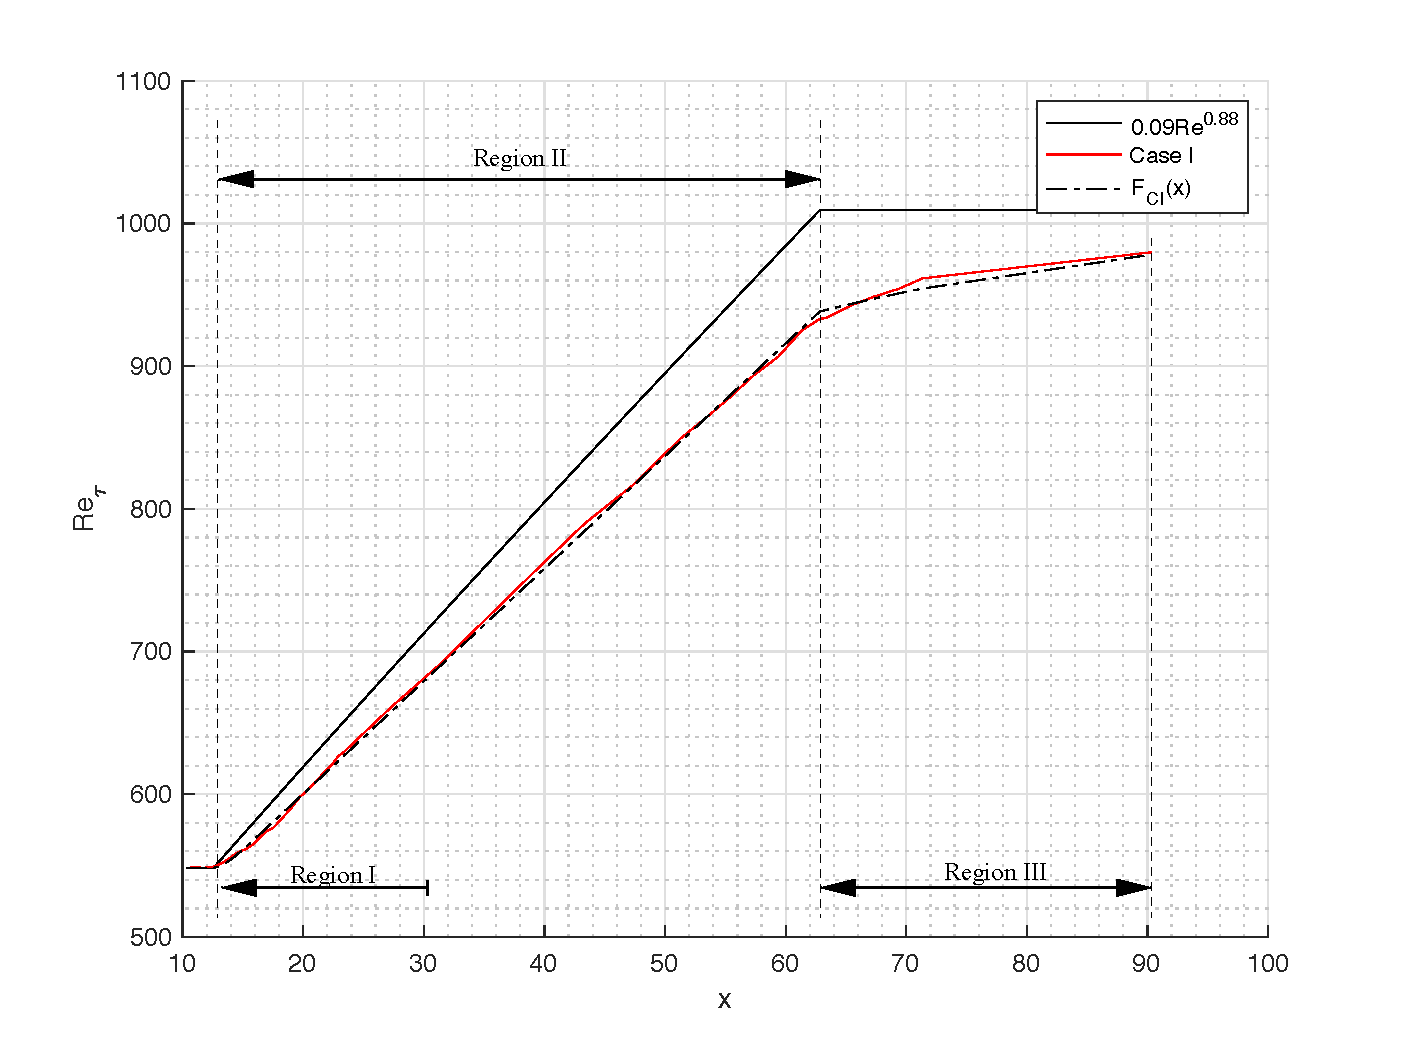
\includegraphics[trim = 20mm 15mm 20mm 10mm, width = 85mm]{convolution_CI.pdf}
\end{center}
  \caption{THE FRICTION REYNOLDS NUMBER THOURGH THE STREAMWISE DIRECTION FOR CASE I.}
  \label{fig:re_t_x}
\end{figure}

\subsubsection*{The friction Reynolds number as a delayed signal.} 



Tab.~\ref{table_conv} shows the important parameters from the convolution functions for each one of the three cases considered in this study.

\begin{table}[t]
\caption{IMPORTANT PARAMETERS FROM THE CASES CONSIDERED.}
\begin{center}
\centering
\label{table_conv}
\begin{tabular}{c l l l l l}
& & & & \\ % put some space after the caption
\hline
Case	&	Region II length	&	\({\delta}_R\)	&	\(R\)	&	\(C\) \\
\hline
I	&	        \(16{\pi}\)	&	\(20{\pi}\)	&	XXX	&	XXX \\
II	&	        \(8{\pi}\)		&	\(12{\pi}\)	&	XXX	&	XXX \\
III	&	        \(4{\pi}\)		&	\(8{\pi}\)	&	XXX	&	XXX \\
\hline
\end{tabular}
\end{center}
\end{table}

\subsection*{Reynolds stresses and turbulent structures}

Fig.~\ref{fig:velocity_CI} shows the instantaneous velocity scalar field in the buffer layer for case I, while Figures from~\ref{fig:u_profile_CI} to~\ref{fig:ww_profile_CI} shows respectively the \(<u>\), \(<uu>\), \(<vv>\) and  \(<ww>\) profiles through the channel for this same case. In all of these plots the \(y^+=30\) turbulent boundary layer is also ploted for this simulation.

\begin{figure*}[h]

%	\scalebox{0.15}
	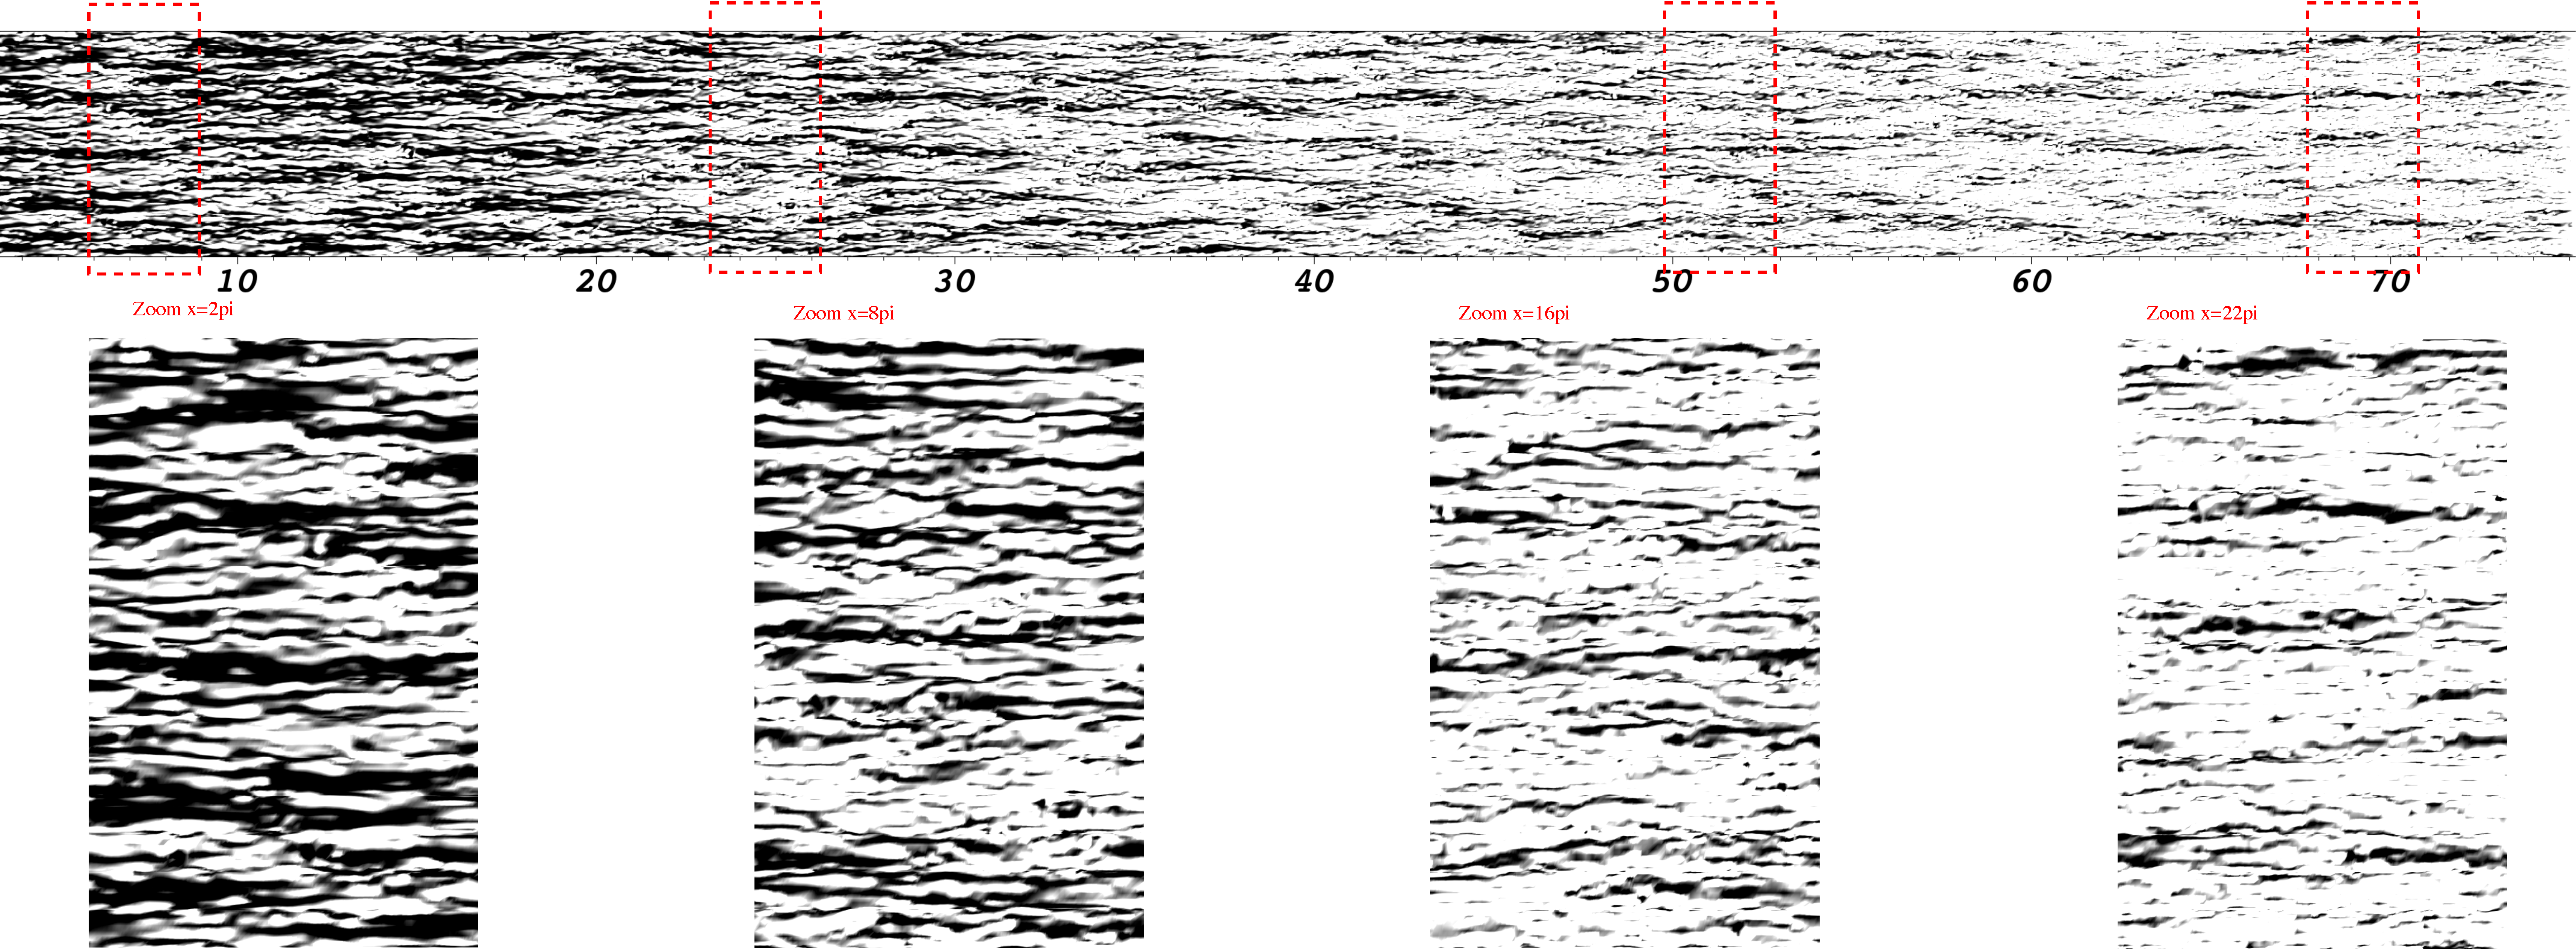
\includegraphics[width=\textwidth]{streaks.pdf}
	\caption{INSTANTANEOUS VELOCITY SCALAR FIELD IN THE BUFFER LAYER FOR CASE I.}
	\label{fig:velocity_CI}
\end{figure*}

\begin{figure}[!htbp]
\begin{center}
\setlength{\unitlength}{0.012500in}%
%  \includegraphics[width=\textwidth, width = 90mm]{u_along_CI.png}
\end{center}
  \caption{\(<u>\) PROFILES THROUGH \(x\) AND \(y^+=30\) TURBULENT BOUNDARY LAYER IN CASE I.}
  \label{fig:u_profile_CI}
\end{figure}

\begin{figure}[!htbp]
\begin{center}
%  \includegraphics[width=\textwidth, width = 90mm]{uu_along_CI.png}
\end{center}
  \caption{\(<uu>\) PROFILES THROUGH \(x\) AND \(y^+=30\) TURBULENT BOUNDARY LAYER IN CASE I.}
  \label{fig:uu_profile_CI}
\end{figure}


Fig.~\ref{fig:velocity_CI} shows the instantaneous velocity scalar field for case I in the Buffer layer, i.e., \(5<y^+<30\)




\bibliography{asme2e}
\appendix   

\end{document}
